\documentclass{standalone}
\begin{document}
\chapter{Pipeline}
The aim of this project is to implement an automated pipeline based on automatic segmentation of T2 weighted Magnetic Resonance (MR) images exploiting Convolutional Neural Networks in order to predict the response to neo-adjuvant chemo-radiotherapy of colorectal cancer using radiomic features.
\begin{figure}[htp]

    \centering
    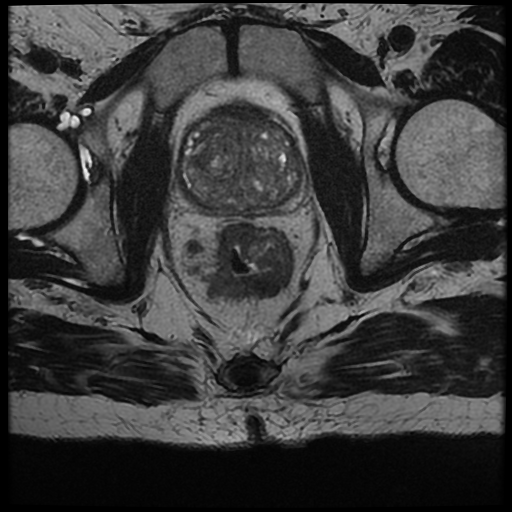
\includegraphics[width=.49\textwidth]{../images/11.png}
    \includegraphics[width=.49\textwidth]{../images/11_contoured.png}
    
    \caption{ \textit{ Left)} Original MRI scan.\textit{ Right)} Segmented colorectal cancer region.}
    \label{comparison}
    
    \end{figure}
    \\
The starting point is the MRI scans. 
Firstly, I stared with the visualization and the pre-processing of the scans.
The processing technique consisted in a smoothing filter to remove noise which could be a potential source of false positive.
The work was then split into two main frameworks.
The former was the \textit{segmentation}, the latter was the \textit{radiomic features} analysis.
The basic idea was to train a Convolutional Neural Network like U-Net, for the segmentation of the scans.
The training process was \textit{supervised}. 
The input images consisted in the MRI scans while as ground-truth the respective medical annotation present in the dataset.
Once trained the model and segmented the images to obtain the colorectal cancer region, the next step was the extraction of the radiomic features.
For each patient's examination in the dataset, I extracted 100 radiomic features.
They were analyzed and processed in order to keep only the most relevant ones.
(La parte sulla features analysis è provvisoria poichè non abbiamo finito il lavoro).
The workflow of the developed pipeline can be seen in Figure\ref{workflow}
\begin{figure}[htp]

    \centering
    \includegraphics[width=\textwidth]{../images/workflow.png}
    
    \caption{Workflow of the developed pipeline. PROVVISORIO}
    \label{workflow}
    
    \end{figure}
    \\
Obviously, the final pipeline structure does not involve a learning process and a feature analysis step since the models are already trained.
As consequence, the final structure of the pipeline looks like in Figure\ref{pipeline}
\begin{figure}[htp]

    \centering
    \includegraphics[width=\textwidth]{../images/pipeline.png}
    
    \caption{final pipeline structure. PROVVISORIO}
    \label{pipeline}
    
    \end{figure}
\end{document}